To show the consequences of violating the assumption of homoscedasticity, a dataset is generated with and without homoscedasticity. It starts with generating four normally distributed independent variables using a random number generator. Then, the dependent variable is generated as a function of the four independent variables. A regression model is fitted, and the model is tested. After this, homoscedasticity is violated by adding an error term that scales with the dependent variable. The model is tested again, and it becomes apparent what the consequences of violating the assumption of homoscedasticity are.

%\lstinputlisting[language=R, caption=super syntetisk data]{kode/super syntetisk data_.R}



\begin{figure}[h] 
	\centering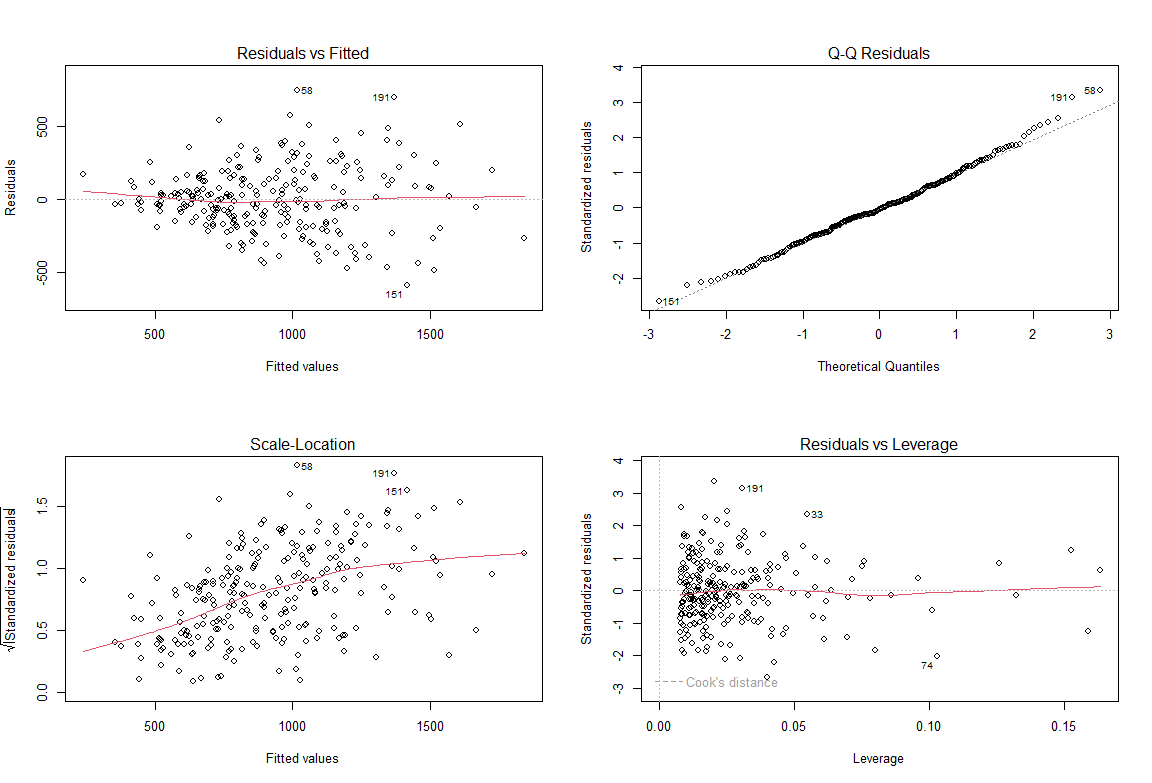
\includegraphics[width=14cm]{billder/4.png}
	\caption{residualplot}
	\label{fig:j06}
\end{figure}

\begin{figure}[h] 
	\centering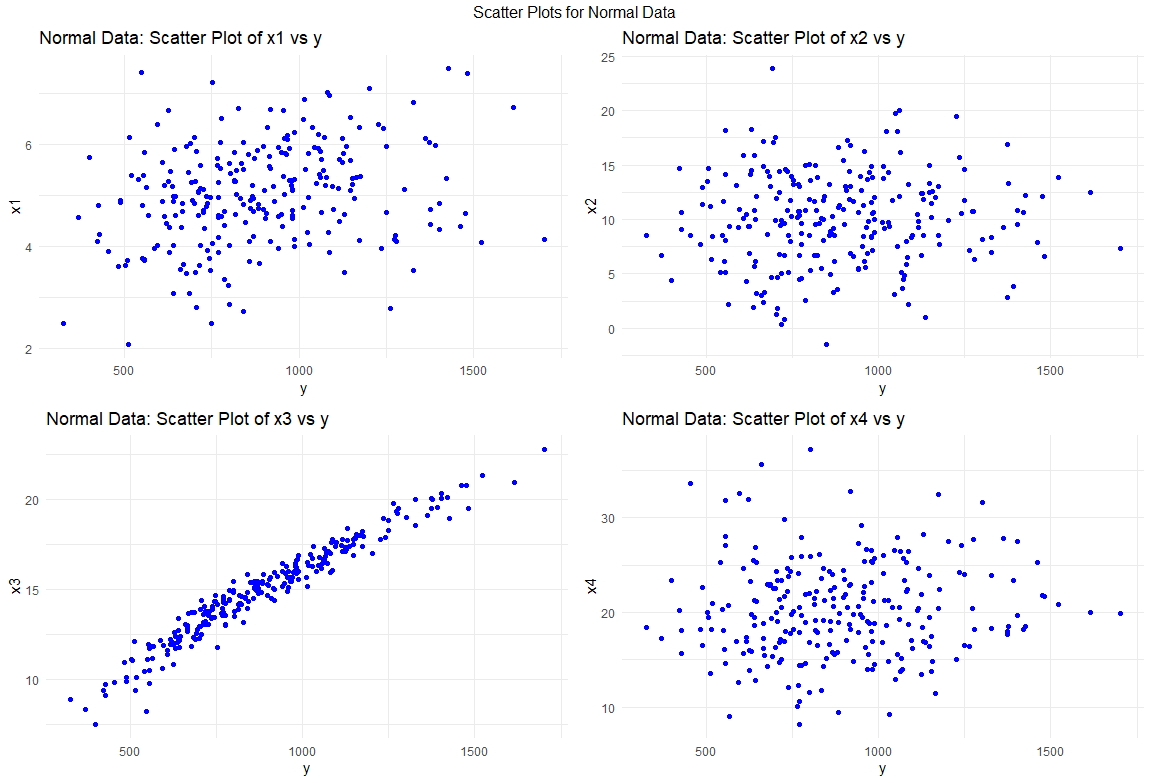
\includegraphics[width=14cm]{billder/5.png}
	\caption{scatterplot.homo}
	\label{fig:j06}
\end{figure}

\begin{figure}[h] 
	\centering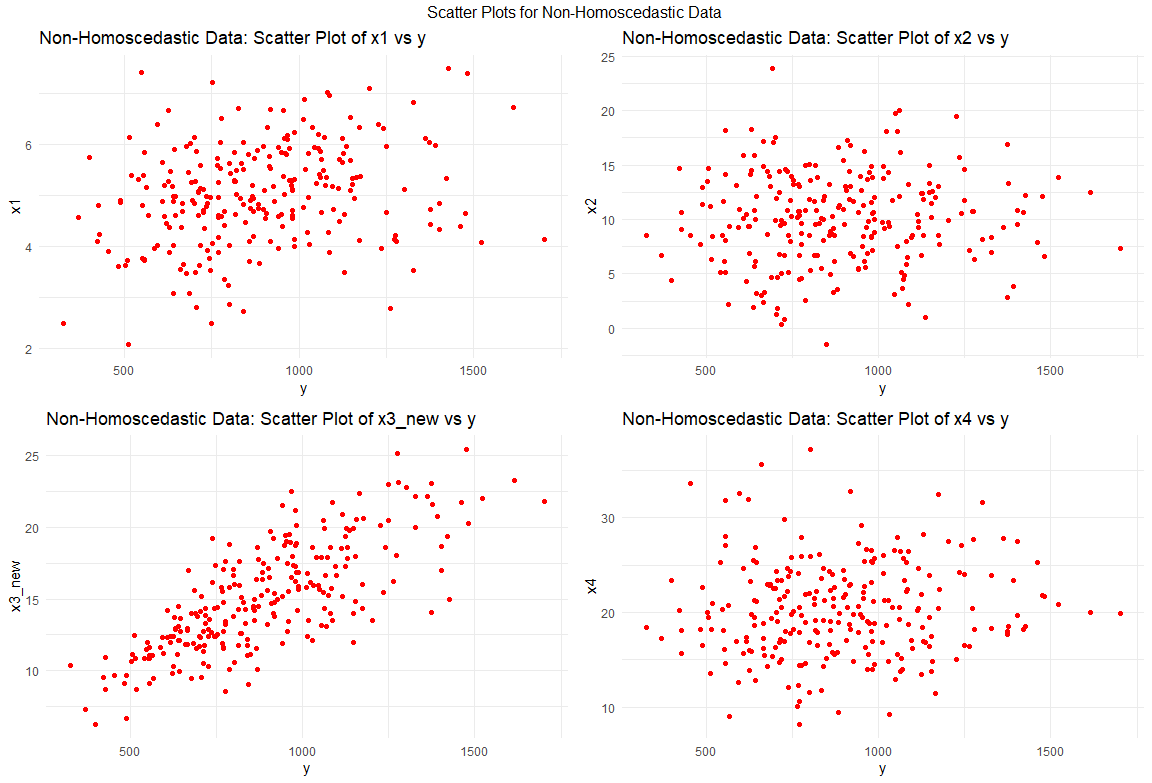
\includegraphics[width=14cm]{billder/6.png}
	\caption{scatterplot.hetro}
	\label{fig:j06}
\end{figure}

\begin{figure}[h] 
	\centering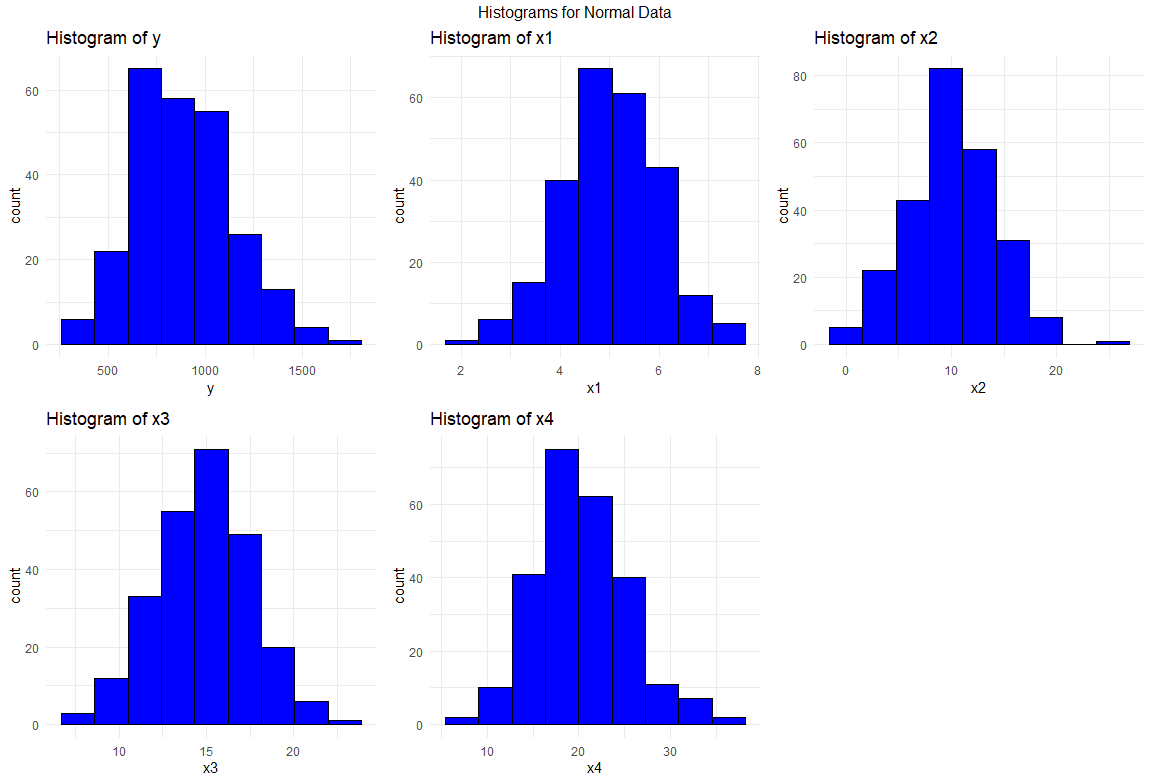
\includegraphics[width=14cm]{billder/7.png}
	\caption{his.homo}
	\label{fig:j06}
\end{figure}

\begin{figure}[h] 
	\centering
	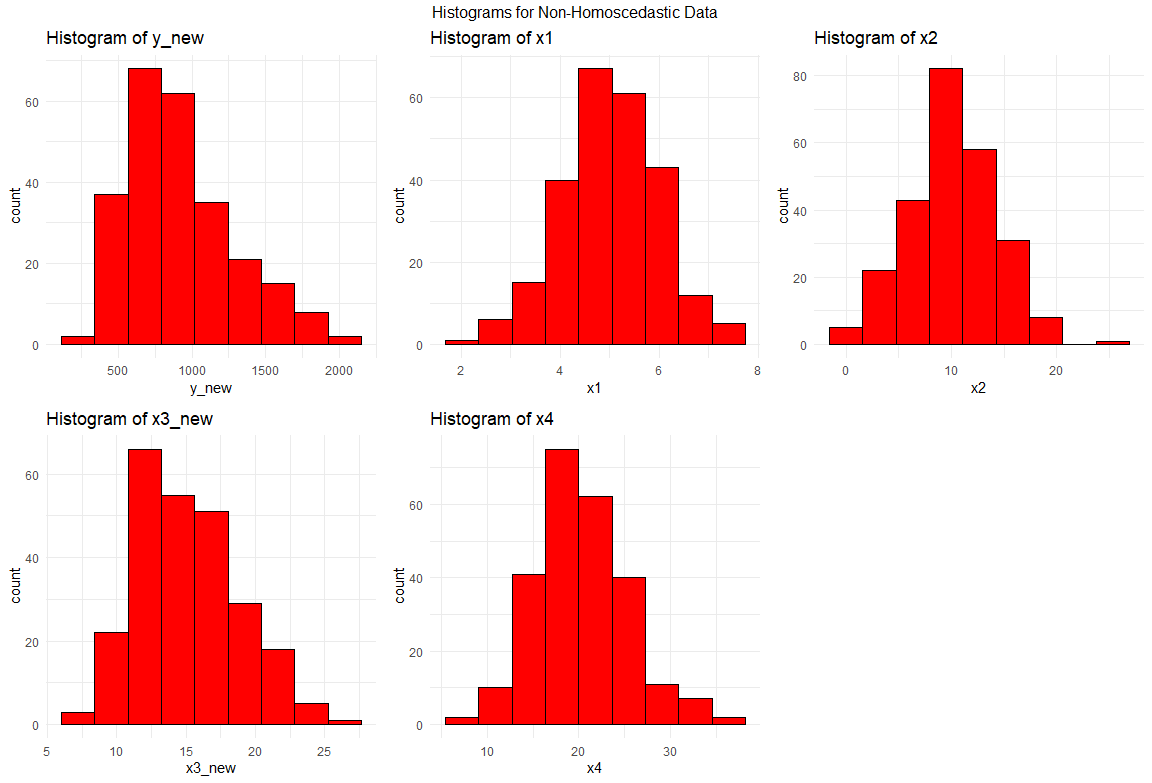
\includegraphics[width=14cm]{billder/8.png}
	\caption{his.hetro.}
	\label{fig:j06}
\end{figure}


%\begin{figure}[h] 
%	\centering
%	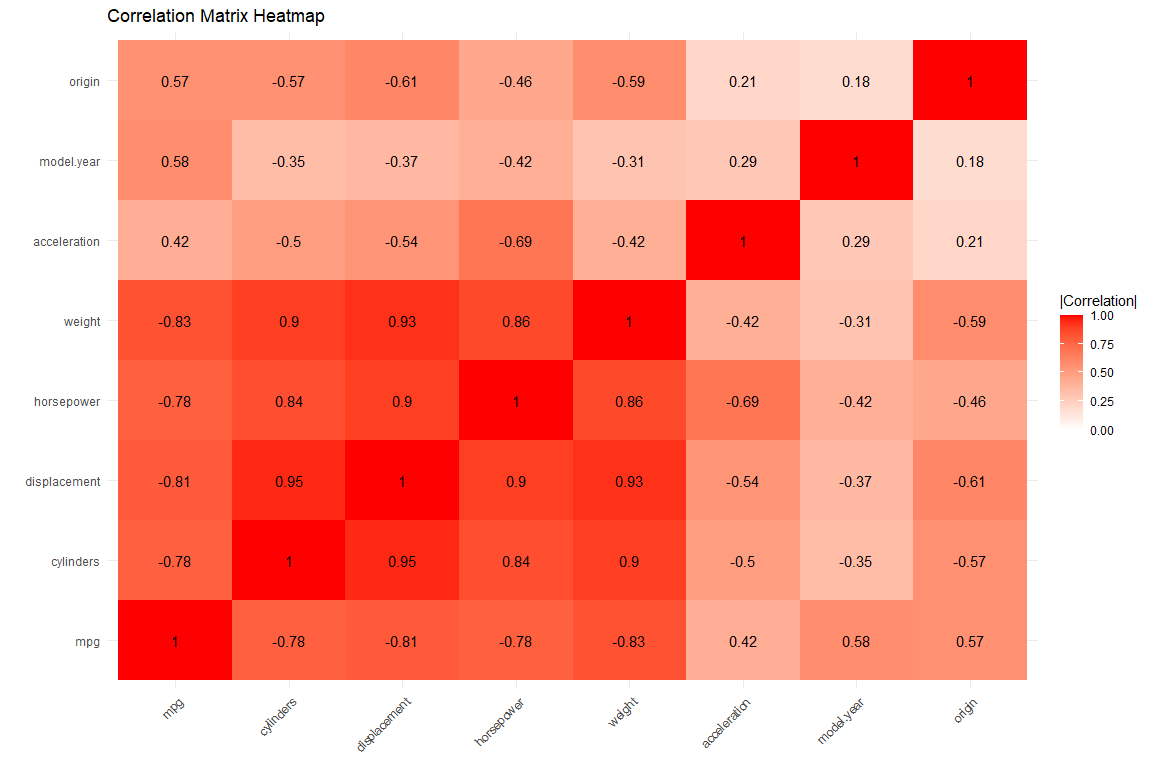
\includegraphics[width=14cm]{1.JPG}
%	\caption{model 1}
%	\label{fig:j06}
%\end{figure}

%\begin{figure}[h] 
%	\centering
%	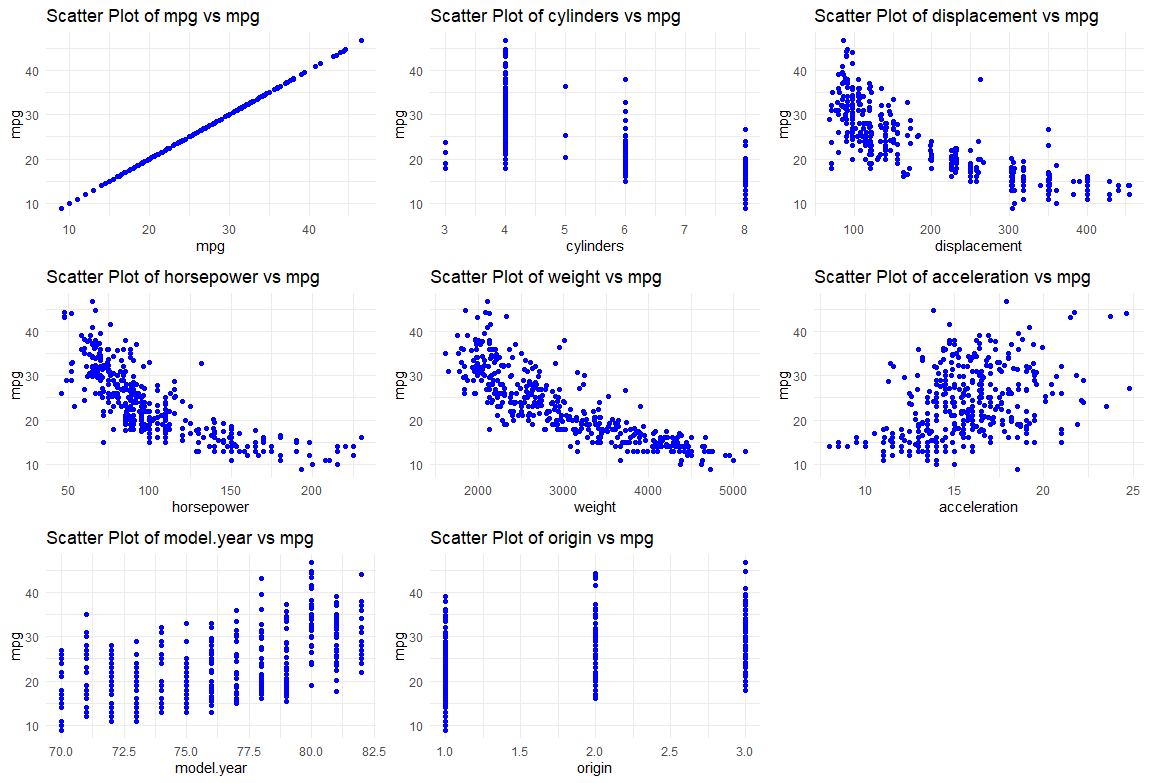
\includegraphics[width=14cm]{2.JPG}
%	\caption{model 2}
%	\label{fig:j06}
%\end{figure}
%
%\begin{figure}[h] 
%	\centering
%	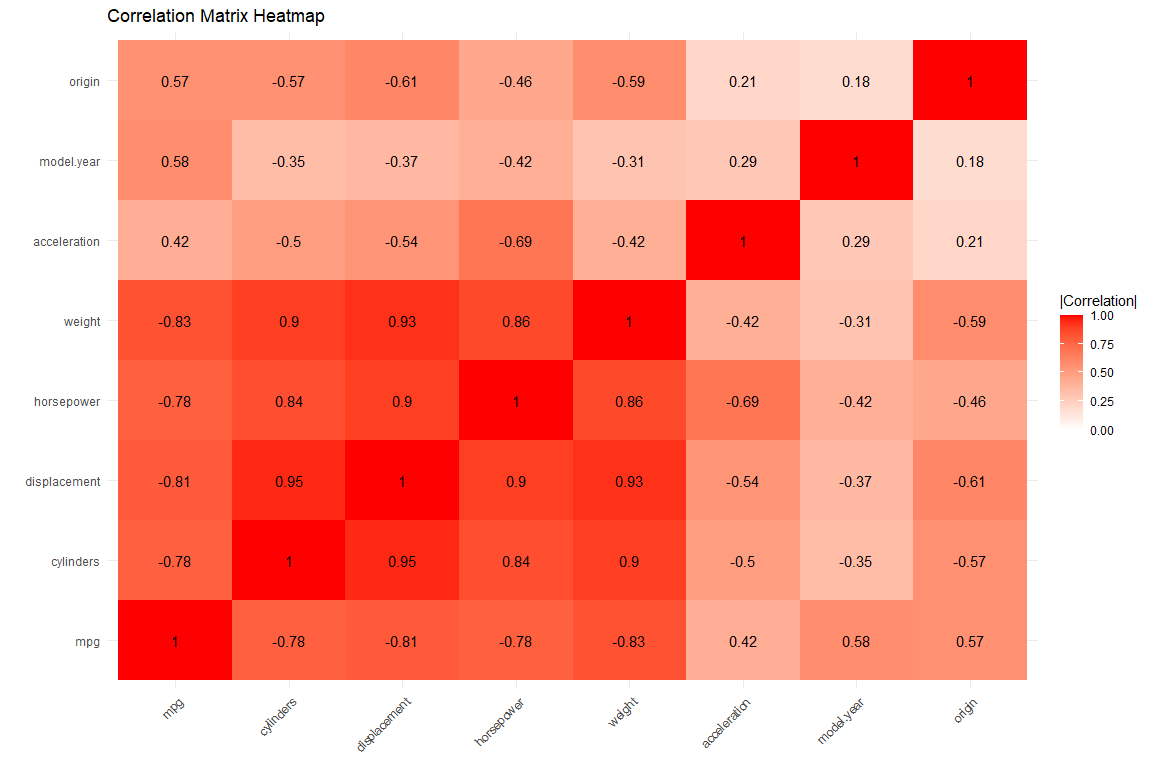
\includegraphics[width=14cm]{1.JPG}
%	\caption{model opsumering 1}
%	\label{fig:j06}
%\end{figure}

%\begin{figure}[h] 
%	\centering
%	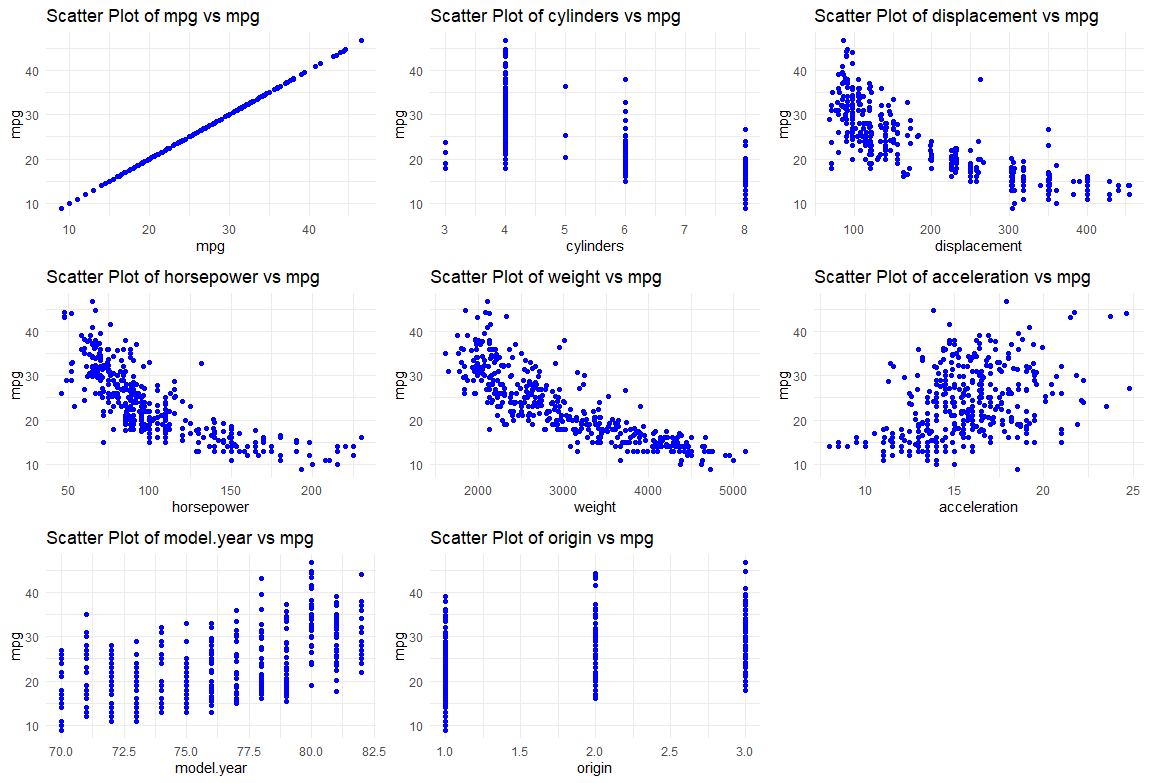
\includegraphics[width=14cm]{2.JPG}
%	\caption{model opsumering 2}
%	\label{fig:j06}
%\end{figure}

